\ifx\wholebook\relax \else

\documentclass[UTF8]{article}
\usepackage[nomarginpar
  %, margin=.5in
]{geometry}

\addtolength{\oddsidemargin}{-0.05in}
\addtolength{\evensidemargin}{-0.05in}
\addtolength{\textwidth}{0.1in}

%
% loading packages
%

\RequirePackage{ifpdf}
\RequirePackage{ifxetex}

%
%
\ifpdf
  \RequirePackage[pdftex,%
       bookmarksnumbered,%
              colorlinks,%
          linkcolor=blue,%
              hyperindex,%
        plainpages=false,%
       pdfstartview=FitH]{hyperref}
\else\ifxetex
  \RequirePackage[bookmarksnumbered,%
               colorlinks,%
           linkcolor=blue,%
               hyperindex,%
         plainpages=false,%
        pdfstartview=FitH]{hyperref}
\else
  \RequirePackage[dvipdfm,%
        bookmarksnumbered,%
               colorlinks,%
           linkcolor=blue,%
               hyperindex,%
         plainpages=false,%
        pdfstartview=FitH]{hyperref}
\fi\fi
%\usepackage{hyperref}

% other packages
%--------------------------------------------------------------------------
\usepackage{graphicx, color}
\usepackage{wrapfig}
\usepackage{subfig}
\usepackage{multicol}
\usepackage{tikz}
\usetikzlibrary{matrix,positioning,shapes}
\usetikzlibrary{patterns}

\usepackage{amsmath, amsthm, amssymb} % for math
\usepackage{exercise} % for exercise
\usepackage{import} % for nested input

%
% for programming
%
\usepackage{verbatim}
\usepackage{fancyvrb}
\usepackage{listings}
%\usepackage{algorithmic} %old version; we can use algorithmicx instead
%\usepackage[plain]{algorithm} %remove rule (horizontal line on top/below the algorithm
\usepackage{algorithm} %to remove rules change to \usepackage[plain]{algorithm}
%\usepackage{algorithm2e}
\usepackage[noend]{algpseudocode} %for pseudo code, include algorithmicsx automatically
\usepackage{appendix}
\usepackage{makeidx} % for index support
\usepackage{titlesec}
\usepackage{epigraph}

\usepackage[cm-default]{fontspec}
\usepackage{xunicode}
%\usepackage{fontenc}
\usepackage{textcomp}
\usepackage{url}

% detect and select Chinese font
% ------------------------------
% fc-list :lang=zh    % list all Chinese fonts
% fc-list :mono       % list all mono fonts
% fc-cache            % refresh cache to load new installed fonts
\def\macmainfont{STSong}  % Under Mac OS X
\def\macmonofont{Monaco}
\def\winmainfont{SimSun} % Under Windows
\def\winmonofont{Consolas}
\def\linuxmainfont{WenQuanYi Micro Hei} % Under Linux
\def\linuxmainfont{Courier}

\suppressfontnotfounderror1 % Avoid setting exit code (error level) to break make process
\count255=\interactionmode
\batchmode

% main font
\let\mainft=\macmainfont
\font\thefont="\mainft"\space at 10pt
\ifx\thefont\nullfont
  \let\mainft=\winmainfont
  \font\thefont="\mainft"\space at 10pt
  \ifx\the\nullfont
    \let\mainft=\linuxmainfont
    \font\thefont="\mainft"\space at 10pt
    \ifx\the\nullfont
      \errorstopmode
      \errmessage{no suitable Chinese main font found}
    \fi
  \fi
\fi

% mono font
\let\monoft=\macmonofont
\font\thefont="\monoft"\space at 10pt
\ifx\thefont\nullfont
  \let\monoft=\winmonofont
  \font\thefont="\monoft"\space at 10pt
  \ifx\the\nullfont
    \let\monoft=\linuxmonofont
    \font\thefont="\monoft"\space at 10pt
    \ifx\the\nullfont
      \errorstopmode
      \errmessage{no suitable mono font found}
    \fi
  \fi
\fi

\interactionmode=\count255

\setmainfont[Mapping=tex-text]{\mainft}
\setmonofont[Scale=MatchLowercase]{\monoft}   % 英文等宽字体

\XeTeXlinebreaklocale "zh"  % to solve the line breaking issue
\XeTeXlinebreakskip = 0pt plus 1pt minus 0.1pt

\titleformat{\paragraph}
{\normalfont\normalsize\bfseries}{\theparagraph}{1em}{}
\titlespacing*{\paragraph}
{0pt}{3.25ex plus 1ex minus .2ex}{1.5ex plus .2ex}

\lstdefinelanguage{Smalltalk}{
  morekeywords={self,super,true,false,nil,thisContext}, % This is overkill
  morestring=[d]',
  morecomment=[s]{"}{"},
  alsoletter={\#:},
  escapechar={!},
  literate=
    {BANG}{!}1
    {UNDERSCORE}{\_}1
    {\\st}{Smalltalk}9 % convenience -- in case \st occurs in code
    % {'}{{\textquotesingle}}1 % replaced by upquote=true in \lstset
    {_}{{$\leftarrow$}}1
    {>>>}{{\sep}}1
    {^}{{$\uparrow$}}1
    {~}{{$\sim$}}1
    {-}{{\sf -\hspace{-0.13em}-}}1  % the goal is to make - the same width as +
    %{+}{\raisebox{0.08ex}{+}}1		% and to raise + off the baseline to match -
    {-->}{{\quad$\longrightarrow$\quad}}3
	, % Don't forget the comma at the end!
  tabsize=2
}[keywords,comments,strings]

% for literate Haskell code
\lstdefinestyle{Haskell}{
  flexiblecolumns=false,
  basewidth={0.5em,0.45em},
  morecomment=[l]--,
  literate={+}{{$+$}}1 {/}{{$/$}}1 {*}{{$*$}}1 {=}{{$=$}}1
           {>}{{$>$}}1 {<}{{$<$}}1 {\\}{{$\lambda$}}1
           {\\\\}{{\char`\\\char`\\}}1
           {->}{{$\rightarrow$}}2 {>=}{{$\geq$}}2 {<-}{{$\leftarrow$}}2
           {<=}{{$\leq$}}2 {=>}{{$\Rightarrow$}}2
           {\ .}{{$\circ$}}2 {\ .\ }{{$\circ$}}2
           {>>}{{>>}}2 {>>=}{{>>=}}2
           {|}{{$\mid$}}1
}

% "define" Scala
\lstdefinelanguage{Scala}{
  morekeywords={abstract,case,catch,class,def,%
    do,else,extends,false,final,finally,%
    for,if,implicit,import,match,mixin,%
    new,null,object,override,package,%
    private,protected,requires,return,sealed,%
    super,this,throw,trait,true,try,%
    type,val,var,while,with,yield},
  otherkeywords={=>,<-,<\%,<:,>:,\#,@},
  sensitive=true,
  morecomment=[l]{//},
  morecomment=[n]{/*}{*/},
  morestring=[b]",
  morestring=[b]',
  morestring=[b]"""
}

\lstloadlanguages{C, C++, Java, Lisp, Haskell, Python, Smalltalk, Scala}

\lstset{
  basicstyle=\small\ttfamily,
  commentstyle=\rmfamily,
  texcl=true,
  showstringspaces = false,
  upquote=true,
  flexiblecolumns=false
}

\newcommand\doubleplus{+\kern-1.3ex+\kern0.8ex}

% ======================================================================

\def\BibTeX{{\rm B\kern-.05em{\sc i\kern-.025em b}\kern-.08em
    T\kern-.1667em\lower.7ex\hbox{E}\kern-.125emX}}

%
% mathematics
%
\newcommand{\be}{\begin{equation}}
\newcommand{\ee}{\end{equation}}
\newcommand{\bmat}[1]{\left( \begin{array}{#1} }
\newcommand{\emat}{\end{array} \right) }
\newcommand{\VEC}[1]{\mbox{\boldmath $#1$}}

% numbered equation array
\newcommand{\bea}{\begin{eqnarray}}
\newcommand{\eea}{\end{eqnarray}}

% equation array not numbered
\newcommand{\bean}{\begin{eqnarray*}}
\newcommand{\eean}{\end{eqnarray*}}

\newtheorem{theorem}{定理}[section]
\newtheorem{lemma}[theorem]{引理}
\newtheorem{proposition}[theorem]{Proposition}
\newtheorem{corollary}[theorem]{Corollary}

% 中文书籍设置
% ====================================
\renewcommand\contentsname{目\ 录}
%\renewcommand\listfigurename{插图目录}
%\renewcommand\listtablename{表格目录}
\renewcommand\figurename{图}
\renewcommand\tablename{表}
\renewcommand\proofname{证明}
\renewcommand\ExerciseName{练习}
%\renewcommand{\algorithmcfname}{算法}

\ifx\wholebook\relax
\renewcommand\bibname{参\ 考\ 文\ 献}                    %book类型
%\newtheorem{Definition}[Theorem]{定义}
\newtheorem{Theorem}{定理}[chapter]
\newtheorem{example}{例题}[chapter]
\else
\renewcommand\refname{参\ 考\ 文\ 献}
\fi

%\setcounter{secnumdepth}{4}
\titleformat{\chapter}
  {\normalfont\bfseries\Large}
  {第\arabic{chapter}章}
  {12pt}{\Large}
%% \titleformat{\subsection}
%%   {\normalfont\bfseries\large}
%%   {\CJKnumber{\arabic{subsection}}、}
%%   {12pt}{\large}
%% \titleformat{\subsubsection}
%%   {\normalfont\bfseries\normalsize}
%%   {\arabic{subsubsection}.}
%%   {12pt}{\normalsize}

%\renewcommand{\baselinestretch}{1.5}                        %文章行间距为1.5倍。

\makeatletter
\newcommand{\verbatimfont}[1]{\renewcommand{\verbatim@font}{\ttfamily#1}}
\makeatother

\setcounter{tocdepth}{4}
\setcounter{secnumdepth}{4}

%\verbatimfont{\footnotesize}


\setcounter{page}{1}

\begin{document}

\title{前言}

\author{刘新宇
\thanks{{\bfseries 刘新宇} \newline
  Email: liuxinyu95@gmail.com \newline}
  }

\maketitle
\fi

\markboth{前言}{编程中的数学}

\chapter*{前言}
%\phantomsection  % so hyperref creates bookmarks
%\addcontentsline{toc}{chapter}{前言}

我讲一个从马爷爷那里听来的故事。有一年春节的时候,北京地坛公园的庙会里人山人海,小朋友们拿着压岁钱在各种摊位上买自己喜欢的玩具。有一个摊位上围了一群人。地上一字排开摆了九个小玩具,每个玩具上依次贴着一元、二元、三元……直到九元的标签。摊主一边向大家吆喝,一边讲解游戏规则:“大家快来玩套圈游戏!一次一元钱,你扔一个,我扔一个,一个玩具只能套一个圈。你要是有三个套中的玩具加到一起值十五元,就可以把玩具都赢走。”

\vspace{5mm}
\begin{tabular}{|c|c|c|c|c|c|c|c|c|}
\hline
1 & 2 & 3 & 4 & 5 & 6 & 7 & 8 & 9 \\
\hline
\end{tabular}
\vspace{5mm}

有个小男孩掏出一元钱,拿了一个红色的圈,使劲一扔。真准!正好套在了七块钱的玩具汽车上,摊主拿出一个蓝色的圈,一下子套中了八块钱的兔爷。

\vspace{5mm}
\begin{tabular}{|c|c|c|c|c|c|c|c|c|}
\hline
1 & 2 & 3 & 4 & 5 & 6 & 7 & 8 & 9 \\
\hline
  &   &   &   &   &   & 男孩 & 摊主 & \\
\hline
\end{tabular}
\vspace{5mm}

小男孩又花了一元钱,这次他套中了价值两元的一个风车,这样只要他下次再套中那个六元的九连环就赢了。可这次摊主不慌不忙地套住了那只九连环。

\vspace{5mm}
\begin{tabular}{|c|c|c|c|c|c|c|c|c|}
\hline
1 & 2 & 3 & 4 & 5 & 6 & 7 & 8 & 9 \\
\hline
  & 男孩  &   &   &   & 摊主  & 男孩 & 摊主 & \\
\hline
\end{tabular}
\vspace{5mm}

这下可糟了,如果接下来摊主再套中那个一元钱的中国结,小男孩就要输了。小男孩涨红了脸,只能抢先去套那个中国结,他试了两次终于套中了。

\vspace{5mm}
\begin{tabular}{|c|c|c|c|c|c|c|c|c|}
\hline
1 & 2 & 3 & 4 & 5 & 6 & 7 & 8 & 9 \\
\hline
男孩  & 男孩  &   &   &   & 摊主  & 男孩 & 摊主 & \\
\hline
\end{tabular}
\vspace{5mm}

摊主接下来扔了一个圈,套住了四元钱的孙悟空面具。小男孩套住了五元钱的小猪存钱罐。

\vspace{5mm}
\begin{tabular}{|c|c|c|c|c|c|c|c|c|}
\hline
1 & 2 & 3 & 4 & 5 & 6 & 7 & 8 & 9 \\
\hline
男孩  & 男孩  &   & 摊主  & 男孩  & 摊主  & 男孩 & 摊主 & \\
\hline
\end{tabular}
\vspace{5mm}

但是摊主扔出一个圈,套住了三元的不倒翁。由于3 + 4 + 8 = 15,小男孩输了。

\vspace{5mm}
\begin{tabular}{|c|c|c|c|c|c|c|c|c|}
\hline
1 & 2 & 3 & 4 & 5 & 6 & 7 & 8 & 9 \\
\hline
男孩  & 男孩  & 摊主  & 摊主  & 男孩  & 摊主  & 男孩 & 摊主 & \\
\hline
\end{tabular}
\vspace{5mm}

周围的人看着很好玩,也纷纷掏钱套圈玩。马爷爷看了一阵,觉得很奇怪,大多数情况下都是摊主赢,偶尔会平局。马爷爷怀疑摊主一定有什么秘密,他只是为了避免人们怀疑,有时才故意输掉游戏。

马爷爷回到家,电视里正在讲中国古老的《河图洛书》,据说在文字尚未发明之前,伏羲治理天下的时候,在黄河支流,有乌龟背负着神秘的图案爬上岸来。如果把图案中的圆点数目用现代的方法表示出来,就是一个数学上的三阶幻方。

\begin{figure}[htbp]
 \centering
 \subcaptionbox{洛书}[0.45\linewidth]{ 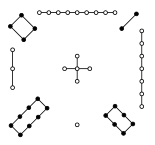
\includegraphics[scale=0.6]{img/luo-shu.png}}
 \subcaptionbox{三阶幻方}[0.45\linewidth]{
   \begin{tabular}{|c|c|c|}
   \hline
   4 & 9 & 2 \\
   \hline
   3 & 5 & 7 \\
   \hline
   8 & 1 & 6 \\
   \hline
   \end{tabular}
   \vspace{8mm}
 }
 \captionsetup{labelformat=empty}
 \caption{}
 \label{fig:luo-shu}
\end{figure}

可别被这个名字吓到,就是方形的九个格子里每行、每列、两个对角线上的三个数字加起来都相等,都等于十五。例如第一行的数字相加是4 + 9 + 2 = 15,第三列的数字相加是2 + 7 + 6 = 15,左上右下的对角线的数字相加是4 + 5 + 6 = 15。等一等——马爷爷想,我现在知道庙会里套圈游戏背后的秘密了。如果要套中的三个玩具加起来等于十五元,那么就相当于套中了幻方的一行、一列、或一个对角线。如果摊主在柜台里偷偷藏一张三阶幻方的图,那么他实际上相当于在和游人玩俗称“一条龙”的井字棋游戏。

\begin{figure}[htbp]
 \centering
 \subcaptionbox{三阶幻方}[0.45\linewidth]{
   \begin{tabular}{|c|c|c|}
   \hline
   4 & 9 & 2 \\
   \hline
   3 & 5 & 7 \\
   \hline
   8 & 1 & 6 \\
   \hline
   \end{tabular}
   \vspace{3mm}
 }
 \subcaptionbox{井字棋游戏}[0.45\linewidth]{
   \begin{tabular}{c|c|c}
   $\times$ &  & $\bigcirc$ \\
   \hline
   $\times$ & $\times$ &  \\
   \hline
   $\bigcirc$ & $\times$ & $\bigcirc$ \\
   \end{tabular}
   \vspace{3mm}
 }
 \captionsetup{labelformat=empty}
 \caption{}
 \label{fig:bingo-magic-square}
\end{figure}

庙会中那个小男孩和摊主的套圈游戏相当于下面的井字棋对局。摊主在关键的第三步中给小男孩设置了一个陷阱,他在第一列上和一个对角线上同时可能连成直线,如果小男孩套中3,则摊主套中5依然能赢。如果了解过博弈游戏,或者知道一点编程,你就知道井字棋游戏没有必胜的策略,如果游戏双方都足够小心,结果一定是平局。偷偷拥有三阶幻方图的摊主这样就站在了不败的地位上,而其他游客一无所知。

\begin{figure}[htbp]
 \centering
 \subcaptionbox{三阶幻方}[0.45\linewidth]{
   \begin{tabular}{|c|c|c|}
   \hline
   4 & 9 & 2 \\
   \hline
   3 & 5 & 7 \\
   \hline
   8 & 1 & 6 \\
   \hline
   \end{tabular}
   \vspace{3mm}
 }
 \subcaptionbox{第一步,男孩套中7,摊主套中8}[0.45\linewidth]{
   \begin{tabular}{c|c|c}
   &  & \\
   \hline
   &  & $\times$ \\
   \hline
   $\bigcirc$ & & \\
   \end{tabular}
   \vspace{3mm}
 } \vspace{3mm} \\
 \subcaptionbox{第二步,男孩套中2,摊主套中6}[0.45\linewidth]{
   \begin{tabular}{c|c|c}
   &  & $\times$\\
   \hline
   &  & $\times$ \\
   \hline
   $\bigcirc$ & & $\bigcirc$ \\
   \end{tabular}
   \vspace{3mm}
 }
 \subcaptionbox{第三步,男孩套中1,摊主套中4}[0.45\linewidth]{
   \begin{tabular}{c|c|c}
   $\bigcirc$ &  & $\times$\\
   \hline
   &  & $\times$ \\
   \hline
   $\bigcirc$ & $\times$ & $\bigcirc$ \\
   \end{tabular}
   \vspace{3mm}
 } \vspace{3mm} \\
 \subcaptionbox{第四步,男孩套中5,摊主套中3,摊主胜}[0.45\linewidth]{
   \begin{tabular}{c|c|c}
   $\pmb{\bigcirc}$ &  & $\times$\\
   \hline
   $\pmb{\bigcirc}$ &  $\times$ & $\times$ \\
   \hline
   $\pmb{\bigcirc}$ & $\times$ & $\bigcirc$ \\
   \end{tabular}
   \vspace{3mm}
 }
 \captionsetup{labelformat=empty}
 \caption{}
 \label{fig:game-steps}
\end{figure}

这个故事是真的么?当然不是,马爷爷是个虚构的人物,他在真实世界中名叫马丁$\cdot$加德纳——举世闻名的美国趣味数学大师。这个故事来自他的《啊哈!灵机一动》。故事不是发生在北京的地坛公园,而是美国的乡村小镇。摊主名叫卡内,而玩游戏的小男孩实际是一位女士。这个游戏也不是中国传统的套圈游戏,而是用硬币盖住一排数字。

这个故事和其中所讲的游戏不断在说着一个重要的概念——同构。一行九个数字和三行三列的格子同构,相加等于15的目标与行、列、对角线同构,古老的《洛书》和数学幻方同构,马爷爷和加德纳同构,中国的春节庙会和美国乡村游乐同构……这其实也是本书想传达的概念,编程和数学同构,和艺术同构,和音乐同构。伟大的发现背后有曲折的故事和性格迥异的数学家。

这个故事还有一层隐喻,问题的表象下隐藏着和它同构的理论实质,我们需要了解抽象的本质而不被具体的现象蒙住眼睛。在人工智能和机器学习日新月异的今天,我们能否还靠着一点点聪明和工程实践继续前行?我们是否要打开那些神秘的黑盒子找到那个指引我们前进的地图?

\vspace{15mm}

二零一九年五月于北京

\ifx\wholebook\relax \else

\expandafter\enddocument
%\end{document}

\fi
